\section{Netzwerkflussprobleme}
\begin{example}
Ausgehend von einer Bananenplantage s sollen alle geernteten Bananen zum Lagerhaus t transportiert werden. Für den Transport stehen Straßen mit $r_1,\ldots,r_p$ $\frac{kg}{n}$ Transportkapazität zu den Seehäfen $A_1,\ldots,A_p$ zu Verfügung. Von den Zielhäfen $B_1,\ldots,B_q$ stehen Transportkapazitäten von $d_1,\ldots,d_q$ $\frac{kg}{n}$ zum Supermarkt t bereit.
Die Transportkapazität zwischen den Seehäfen werden mit $c(A_i,A_j), 1\le i\le p, 1\le j \le p$ bezeichnet.
\paragraph{Fragen:}
\begin{itemize}
	\item Ist es mögliche, alle Transportkapazitäten auszuschöpfen?
	\item Falls nein, was ist die maximal mögliche Transportkapazität?
	\item Wie sollen die Bananenladungen aufgeteilt werden?
\end{itemize}
Konstruiere einen gewichteten Digraph $G=(V,E,w)$ mit
\begin{itemize}
	\item $V=\{s, A_1,\ldots,A_p, B_1,\ldots,q,t\} $ 
	\item $E= \{(s,A_i), (A_i,B_j), (B_j,t) ; 1\le i\le p, 1\le j\le p\} $ 
	\item $w(e)= \begin{cases}
			r_i &, e=(s,A_i) \\
			c(A_i,B_j) &, e(A_i,B_j) \\
			d_i &, e(B_i,t)
	\end{cases}$ 
\end{itemize}

\begin{center}
\begin{tikzpicture}


	%Netzwerk einfügen


\end{tikzpicture}
\end{center}
\end{example}
\begin{definition}
Ein \emph{Netzwerk} ist ein Tupel $N=(V,E,c,s,t)$  bestehend aus
\begin{itemize}
	\item einem gewichteten Digraphen $G=(V,E,c)$
	\item einer \emph{Kapazitätsfunktion} $c \colon E \to R_{\ge 0}$
	\item einer Quelle $s \in V$ mit $pre(s)= \emptyset$ 
	\item einer Senke $t \in V$ mit $post(t)=\emptyset$ 
\end{itemize}
Ein Fluss $f \colon E \to R_{\ge 0}$ ist eine Funktion, die folgende Bedingungen erfüllt:
\begin{enumerate}
	\item \emph{Kapazitätsbedingung:}
		\[
		f(v,w) \le c(v,w)
		\]
	\item \emph{Kirchhoffsches Gesetz:}
		\[
		\sum_{u \in pre(v)} f(u,v) = \sum_{w \in  post(v)} f(v,w)
		\]
für alle $v \in V \setminus \{s,t\} $ .
\end{enumerate}
Der \emph{Wert} des Flusses ist:
\[
flow(f) = \sum_{w \in post(s)}f(s,w)
\]
Der \emph{maximale FLuss} von N wird bezeichnet als:
\[
MaxFlow(N) = \max \{flow(f) \text{ ist Fluss für N}\} 
\]
Eine Flussfunktion $f$ wird \emph{optimal} genannt, falls 
\[
flow(f)=MaxFlow(N)
\]
ist. \\
Ein \emph{Schnitt} für N ist eine Knotenmenge $S \subset V$ mit $s \in S, t \not\in S$. \\
Die \emph{Kapazität} eines Schnittes ist gegeben durch:
\[
cap(S)= \sum_{v \in S \\ w \in post(v) \setminus S}c(v,w)
\]
Die minimale Schnittkapazität von N ist:
\[
MinCut(N)= \min \{cap(S) | \text{ S ist Schnitt für N}\} 
\]
\end{definition}
\begin{lemma}
	Sei S ein Schnitt für $N=(V,E,c,s,t)$. Dann gilt für jeden Fluss f, dass
	\begin{align*}
		flow(f) &= \sum_{w \in post(v) \setminus S} f(v,w) - \sum_{u \in  pre(v)} f(u,v) \\
		flow(f) &\le cap(S)
	\end{align*}
\end{lemma}
\begin{proof}
Rechne:
\begin{align*}
	flow(f) &= \sum_{w \in post(s)} f(s,w) \\
		&= \sum_{v \in S}\left( \sum_{w \in post(v)}f(v,w)- \sum_{u \in pre(v)}f(u,v) \right)\\
		&=\sum_{w \in post(v)}f(v,w) - \sum_{u \in pre(v) \setminus S}f(u,v)
\end{align*}
Für die nächste Behauptung können wir ebenfalls nachrechnen:
\begin{align*}
	flow(f) &= \sum_{w \in post(v) \setminus S} f(v,w) - \sum_{u \in pre(v) \setminus S}f(u,v) \\
		&\le \sum_{w \in post(v) \setminus S}c(v,w) \\
		&=cap(S)
\end{align*}
\end{proof}
\begin{theorem}[Max-FLow-Min-Cut Theorem]
\label{thm:min-cut}
Sei $N=(V,E,c,s,t)$ ein Netzwerk, dann gilt:
\[
MaxFlow(N)=MinCut(N)
\]
\end{theorem}
\begin{proof}
\underline{Zu zeigen:} Es gibt einen Schnitt für den die Gleichheit gilt. \\
\underline{Idee:} Gegeben sei ein Fluss f mit flow(f)=MaxFlow(N), konsturiere einen Schnitt $S$ mit flow(f)=cap(S). \\
\begin{algorithm}[H]
\label{alg:beweis-max-min}
\KwData{Netzwerk $N$, Fluss $f$ mit $flow(f)=MaxFlow(N)$.}
\KwResult{S mit $flow(f)=cap(S)$}
\begin{itemize}
	\item $S=\{s\}$ 
	\item \While{$x \in S, y \in V \setminus S$ existieren mit $\begin{cases}
				f(x,y) < c(x,y) &, \text{ falls } (x,y) \in E \\
				0 < f(y,x) &, \text{ falls } (y,x) \in E
	\end{cases}$ \\ dann }{$S=S \cup \{y\}$}
\end{itemize}
\end{algorithm}
\underline{Behauptung} Das Resultat $S$ des Algorithmus ist ein Schnitt von $N$
\begin{proof}
Zu Zeigen: $t \not\in S$ \\
\underline{Angenommen:}  $t \in S, v_r=t$ \\
$\implies$ Es gibt $v_{r-1} \in S$ mit $f(v_{r-1},v_r) < c(v_{r-1},v_r)$. \\
Iterativ: Es gibt einen ungerichteten Weg $\pi$ mit $v_0=s, v_r=t$\\
Definiere für $i=0,\ldots,r-1$:
\[
\varepsilon_i = \begin{cases}
	c(e)-f(e) &, \text{ falls } e=(v_i,v_{i+1}) \in E , e^{-1}=(v_{i+1}, v_i) \not\in E \\
	f(e^{-1}) &, \text{ falls } e \not\in E , e^{-1} \in E \\
	\max \{c(e)-f(e), f(e^{-1})\} &, \text{ falls } e \in E , e^{-1} \in E
\end{cases}
\]
Beobachte: $\varepsilon_i > 0$
\begin{equation}
	\label{eqn:epsilon}
\varepsilon = \min_{ß\le i \le r-1} \varepsilon_i > 0
\end{equation}
\underline{Zeige:} Es gib einen Fluss $f^{*}$ in $N$  mit $flow(f^{*}) = flow(f)+\varepsilon$ \\
\underline{Konstruiere:}
\[
f^{*}(e)= \begin{cases}
	f(e)+\varepsilon &, \text{ falls } e=(v_i, v_{i+1} \in E, e^{-1}\not\in E \\
	f(e)-\varepsilon &, \text{ falls } e = (v_{i+1}, v_i) \in E, e^{-1}\not\in E \\
	f(e)+\varepsilon &, \text{ falls } e=(v_i, v_{i+1}), e^{-1} \in E \text{ und } c(e)-f(e) > f(e^{-1}) \\
	f(e)-\varepsilon &, \text{ falls } e=(v_{i+1}, v_i), e^{-1} \in E \text{ und } c(e)-f(e) \le f(e^{-1}) \\
	f(e) &, \text{ sonst}
\end{cases}
\]
Bemerke:
\begin{itemize}
	\item Kapazitätsbedingung bleibt erfüllt.
	\item Kirchpffsches Gesetz bleibt erfüllt, da $f^{*}$ weiterhin ein Fluss ist.
\end{itemize}
Das heißt:
\begin{align*}
	flow(f^{*}) &= \sum_{v \in post(s)} f^{*}(s,v) \\
		    &= \sum_{v \in pre(t)} f^{*}(v,t) \\
		    &= \sum_{v \in pre(t) \setminus \{v_{r-1}\} } f^{*}(v,t) + f^{*}(v_{r-1},t) \\
		    &=flow(f) +\varepsilon
\end{align*}
Dies ist ein Widerspruch dazu, dass $flow(f) = MaxFlow(N) \implies S$ ist ein Schnitt.
\end{proof}
S ist ein Schnitt in N mit:
\[
f(x,y)=c(x,y) 
\]
\[
	f(y,x)=0
\]
für alle $x \in S, y \in V \setminus S \implies flow(f)=cap(S)$ nach Kirchoff. 
\end{proof}
Wir formalisieren nun weiter:
\begin{definition}
Sei f ein Fluss im Netzwerk $N=(V,E,c,s,t)$. Eine Kante $e=(x,y) \in E$  heißt \emph{Vorwärtskante}, falls $f(e)<c(e)$ \\
Eine Kante $e^{-1}(y,x) \in E$ heißt \emph{Rückwärtskante}, falls $f(e^{-1}) > 0$. \\
Der \emph{Restgraph} für f ist der Digraph $G'=(V,E')$ mit
\[
E'=\{(x,y) \in V \times V | (x,y) \text{ ist Vorwärts- oder Rückwärts-Kante}\} 
\]
$c(e)-f(e)$ bzw. $f(e^{-1})$ heißen \emph{Restkapazitäten}. Ein \emph{augmentierender Weg} ist ein s-t-Weg im Restgraphen.
\end{definition}
Im vorherigen Beweis haben wir einen solchen augmentierenden Weg konstruiert.

\begin{example}
Betrachte
\begin{center}
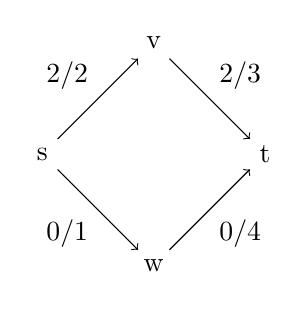
\begin{tikzpicture}[node distance = 2cm, auto]
 \node (v) {v};
 \node (s) [below left of=v] {s};
 \node (w) [below right of=s] {w};
 \node (t) [below right of=v] {t};

 \path [->] (v) edge node[above right]{2/3} (t);
 \path [->] (s) edge node[above left] {2/2}(v);
 \path [->] (s) edge node[below left] {0/1} (w);
 \path [->] (w) edge node[below right] {0/4} (t);
\end{tikzpicture}
\end{center}
Der Restgraph mit Restkapazitäten ist:
\begin{center}
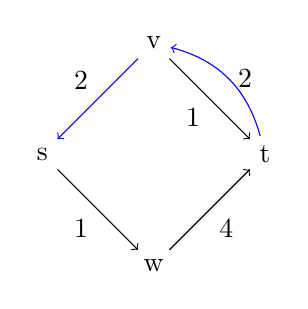
\begin{tikzpicture}[node distance = 2cm, auto]

	\node (v) {v};
 \node (s) [below left of=v] {s};
 \node (w) [below right of=s] {w};
 \node (t) [below right of=v] {t};
\begin{scope}[every edge/.style={draw=blue}]
 \path [->] (t) edge[bend right=30] node[right] {2} (v);
 \path [<-] (s) edge node[above left] {2}(v);
 \end{scope}
 \begin{scope}[ever edge/.style={draw=red}]
 \path [->] (s) edge node[below left] {1} (w);
 \path [->] (w) edge node[below right] {4} (t);
 \path [->] (v) edge node[below left]{1} (t);
\end{scope}
\end{tikzpicture}
\end{center}
Blau: Rückwärtskante, Rot: Vorwärtskante
\end{example}
Der Beweis von Satz \ref{thm:min-cut} gibt uns außerdem einen Algorithmus, wie wir, für einen nicht-optimalen Fluss, ein Fluss mit höheren Wer finden können.
\underline{Idee:} Benutze dies um einen optimalen Fluss zu finden. \\
\begin{algorithm}[H]
	\label{alg:ford-fulkerson}
	\caption{Ford-Fulkerson}
	\KwData{Netzwerk $N=(V,E,c,s,t)$ }
	\KwResult{Fluss $f$ mit $flow(f)=MaxFlow(N)$ }
	\begin{itemize}
		\item $f(e)=0, e \in E$ 
		\item Suche einen augmentierenden Weg von $s$ nach $t$ 
		\item \If{ keiner existiert}{stop}
		\item Berechne $\varepsilon$ \eqref{eqn:epsilon}
		\item Augmentiere $f$ um $\varepsilon$, gehe zu 2
	\end{itemize}
\end{algorithm}
\begin{remark}
Im Falle von irrationalen Kapazitäten muss der Algorithmus nicht notwendigerweise terminieren (Beweis durch Gegenbeispiel)
\end{remark}
\begin{theorem}[Integral-Flow-Theorem]
Sei $N=(V,E,c,s,t)$ ein Netzwerk mit ganzzahligen Kapazitäten. Dann terminiert der Algorithmus \ref{alg:ford-fulkerson} nach maximal $\sum_{e \in E}c(e)$ Augmentierungsschritten mit einem ganzzahligen, optimalen Fluss.
\end{theorem}
\begin{proof} Betrachte:
\paragraph{Ganzzahlig:} Wir starten mit $f(e)=0, e \in E$. Die Restkapazitäten im Algorithmus und somit auch $\varepsilon $ sind zu jedem Zeitpunkt ganzzahlig.
\paragraph{Optimal:} Der Algorithmus terminiert, falls kein augmentierender Weg mehr gefunden werden kann. Der Beweis des Max-Flow-Min-Cut-Theorem zeigt, dass dies den maximalen Fluss impliziert.
\paragraph{Anzahl Schritte} Im schlimmsten Fall wird pro Iteration der Fluss von genau einer Kante um 1 erhöht $\implies$ Behauptung 
\end{proof}
%Beispiel

Es gibt eine Möglichkeit, die Laufzeit des Algorithmus zu verbessern, indem man immer den kürzesten augmentierenden Weg wählt. Dies bringt uns zum nächsten Algorithmus:

